\documentclass[11pt,reqno]{amsart}
\usepackage[T1]{fontenc}
\usepackage[utf8]{inputenc}
\usepackage[spanish,es-noquoting,es-tabla,es-nodecimaldot]{babel}
\usepackage{lmodern,microtype}
\usepackage{amsmath,amssymb,amsthm,mathtools,mathrsfs}
\usepackage[a4paper,margin=2.65cm]{geometry}
\usepackage[hidelinks]{hyperref}
\usepackage{xcolor}
\usepackage{listings}
\usepackage{booktabs}
\usepackage{enumitem}
\usepackage{graphicx}
\definecolor{resultblue}{RGB}{12,54,139}
\definecolor{codegray}{RGB}{75,75,75}
\lstdefinestyle{pyclean}{language=Python,basicstyle=\ttfamily\footnotesize,breaklines=true,breakatwhitespace=true,columns=fullflexible,keepspaces=true,showstringspaces=false,frame=single,framerule=.3pt,rulecolor=\color{black!30},numbers=left,numberstyle=\tiny\color{codegray},numbersep=8pt,keywordstyle=\color{resultblue},commentstyle=\color{codegray},stringstyle=\color{black},tabsize=4}
\newtheorem{theorem}{Teorema}[section]
\newtheorem{proposition}[theorem]{Proposición}
\newtheorem{lemma}[theorem]{Lema}
\newtheorem{corollary}[theorem]{Corolario}
\theoremstyle{definition}\newtheorem{definition}[theorem]{Definición}
\theoremstyle{remark}\newtheorem{remark}[theorem]{Observación}
\DeclareMathOperator{\VaR}{VaR}
\DeclareMathOperator{\ES}{ES}
\newcommand{\E}{\mathbb E}
\newcommand{\Prob}{\mathbb P}
\newcommand{\R}{\mathbb R}
\newcommand{\pos}[1]{(#1)^+}
\newcommand{\resultado}[1]{\ensuremath{{\color{resultblue}\boldsymbol{#1}}}}
\title[Soluciones de los problemas propuestos]{Optimización del reaseguro catastrófico de exceso de pérdida\\\large Soluciones detalladas de los problemas propuestos}
\author{Notas de investigación y docencia}
\date{13 de noviembre de 2026}
\begin{document}
\begin{abstract}
Se resuelven con detalle los siete problemas propuestos en las notas \emph{Optimización del reaseguro catastrófico de exceso de pérdida}. Los problemas 1 a 6 tienen solución analítica; cada cuenta se comprueba con el programa \texttt{soluciones\_problemas.py} (apéndice). El problema 7 se resuelve con dos bases reales: los incendios daneses de Copenhagen Re (1980--1990) y los ciclones tropicales registrados por el CENAPRED en México (2000--2024). Las instrucciones para descargar los datos están en \texttt{DATOS.md}, en la raíz del repositorio.
\end{abstract}
\maketitle
\tableofcontents

\section*{Notación común}
En los problemas 1 a 6 se usa la ley de las notas,
\begin{equation}\label{eq:law}
\begin{array}{c|rrrr}
x_i&0&500&1500&3128\\\hline
p_i&0.70&0.15&0.10&0.05
\end{array}
\qquad \E X=381.40,
\end{equation}
la capa $R_{d,m}(x)=\min\{\pos{x-d},m\}$, la retención $N_{d,m}(x)=x-R_{d,m}(x)$, la tarifa $\Pi(d,m)=(1+\theta)\E R_{d,m}(X)+\gamma m$ y el costo $J(d,m)=\E X+\theta\E R_{d,m}(X)+\gamma m$, con $\theta=0.25$, $\gamma=0.01$ y $\alpha=0.95$. Todos los montos están en millones de pesos.

Un hecho se usa una y otra vez. Como $N_{d,m}$ es no decreciente y el escenario superior tiene probabilidad exactamente $1-\alpha=0.05$,
\begin{equation}\label{eq:esmax}
\ES_{0.95}\bigl(N_{d,m}(X)\bigr)=N_{d,m}(3128)\qquad\text{para todo }(d,m).
\end{equation}

\section{Problema 1: la capa $(d,m)=(500,1500)$}
\emph{Enunciado.} Calcule la recuperación y la retención para $(d,m)=(500,1500)$ y explique la pérdida que queda por encima de la capa.

\emph{Solución.} La capa cubre el tramo $(500,2000]$. Por escenario:
\begin{center}
\begin{tabular}{rrrrl}
\toprule
$x$ & $p$ & $R_{500,1500}(x)$ & $N_{500,1500}(x)$ & región \\
\midrule
0 & 0.70 & 0 & 0 & bajo la prioridad\\
500 & 0.15 & 0 & 500 & justo en la prioridad\\
1500 & 0.10 & 1000 & 500 & dentro de la capa\\
3128 & 0.05 & 1500 & 1628 & capa agotada\\
\bottomrule
\end{tabular}
\end{center}
Hay dos lecturas del escenario $x=500$. Formalmente $R(500)=\min\{0,1500\}=0$: una pérdida igual a la prioridad no activa la capa. Económicamente, la cedente retiene toda la pérdida.

Los momentos son
\begin{align*}
\E R&=0.10(1000)+0.05(1500)=\resultado{175.00},&
\E N&=381.40-175.00=\resultado{206.40},\\
\Pi&=1.25(175)+0.01(1500)=\resultado{233.75},&
J&=206.40+233.75=\resultado{440.15}.
\end{align*}
Como control, la fórmula de supervivencia da lo mismo: $\overline F(t)=0.15$ en $[500,1500)$ y $0.05$ en $[1500,2000)$, así que $\int_{500}^{2000}\overline F=1000(0.15)+500(0.05)=175$.

\emph{La pérdida por encima de la capa.} En $x=3128$ la capa se agota en $d+m=2000$ y la cedente retiene
\[
N(3128)=\underbrace{500}_{\text{prioridad}}+\underbrace{3128-2000}_{\text{exceso sobre }d+m}=500+1128=\resultado{1628}.
\]
Por \eqref{eq:esmax}, $\ES_{0.95}(N)=\resultado{1628}$. El contrato es más barato que el óptimo del Teorema de las notas ($J=440.15<475.73$), pero deja sin proteger justo el escenario que define la cola. Un límite corto produce \emph{agotamiento vertical}: la cobertura funciona en pérdidas medianas y desaparece cuando más se necesita. Para cumplir $\ES_{0.95}(N)\le380$ se necesitan $d\le380$ y $d+m\ge3128$ (Problema 3), y $(500,1500)$ viola ambas condiciones.

\section{Problema 2: prima pura sin Tonelli}
\emph{Enunciado.} Demuestre directamente, sin utilizar Tonelli, que $\E R_{d,m}(X)=\int_d^{d+m}\overline F_X(t)\,dt$ cuando $X$ tiene soporte finito. Relacione los sumandos con los intervalos de supervivencia.

\begin{proposition}
Sea $X$ con valores $0\le a_1<a_2<\dots<a_n$ y probabilidades $p_1,\dots,p_n>0$. Entonces $\E R_{d,m}(X)=\int_d^{d+m}\overline F_X(t)\,dt$.
\end{proposition}
\begin{proof}
\emph{Paso 1 (una pérdida fija).} Para $a\ge0$, la función $t\mapsto\mathbf 1\{a>t\}$ vale $1$ en $[0,a)$ y $0$ después. Su integral de Riemann sobre $[d,d+m]$ es la longitud de $[d,d+m]\cap[0,a)$:
\[
\int_d^{d+m}\mathbf 1\{a>t\}\,dt=\max\{0,\min\{a,d+m\}-d\}=\min\{\pos{a-d},m\}=R_{d,m}(a).
\]
La penúltima igualdad se ve por casos: si $a\le d$ ambos lados son $0$; si $d<a\le d+m$ ambos valen $a-d$; si $a>d+m$ ambos valen $m$.

\emph{Paso 2 (linealidad de una suma finita).} Como $\overline F_X(t)=\sum_{i=1}^n p_i\mathbf 1\{a_i>t\}$ es una suma \emph{finita} de funciones escalonadas, la linealidad de la integral de Riemann permite integrar término a término sin ningún teorema de intercambio:
\[
\int_d^{d+m}\overline F_X(t)\,dt=\sum_{i=1}^n p_i\int_d^{d+m}\mathbf 1\{a_i>t\}\,dt=\sum_{i=1}^n p_i R_{d,m}(a_i)=\E R_{d,m}(X).\qedhere
\]
\end{proof}

\emph{Lectura por intervalos de supervivencia.} Sea $a_0=0$ y sean $I_j=[a_j,a_{j+1})$. En $I_j$ la supervivencia es constante, $\overline F_X(t)=\Prob(X>a_j)=\sum_{i>j}p_i$. Entonces
\begin{equation}\label{eq:intervals}
\E R_{d,m}(X)=\sum_{j}\Prob(X>a_j)\,\bigl|I_j\cap[d,d+m]\bigr|.
\end{equation}
Cada sumando es \emph{(probabilidad de alcanzar ese tramo) $\times$ (longitud del tramo que cae dentro de la capa)}. La capa vende, millón por millón, la probabilidad de que la pérdida llegue a ese millón. Para el contrato del Teorema, $(380,2748)$:
\[
\underbrace{0.30\,(500-380)}_{[380,500)}+\underbrace{0.15\,(1500-500)}_{[500,1500)}+\underbrace{0.05\,(3128-1500)}_{[1500,3128)}=36+150+81.4=\resultado{267.40},
\]
que coincide con $\E R=267.40$ de las notas. Las dos sumas reordenan los mismos términos: la del paso 2 recorre escenarios (renglones) y \eqref{eq:intervals} recorre tramos de pérdida (columnas).

\section{Problema 3: otros presupuestos de riesgo}
\emph{Enunciado.} Repita la optimización para $B\in\{250,380,600\}$ y determine, con demostración, si las fórmulas del Teorema siguen siendo válidas.

\begin{theorem}\label{thm:B}
Para todo $B\in[0,3128)$, el problema $\min_{d,m\ge0}J(d,m)$ sujeto a $\ES_{0.95}(N_{d,m}(X))\le B$ tiene la solución única
\[
\resultado{d^*(B)=B,\qquad m^*(B)=3128-B.}
\]
Si $B\ge3128$, la restricción no obliga a nada y la solución es $m^*=0$ (no reasegurar).
\end{theorem}
\begin{proof}
\emph{Región factible.} Por \eqref{eq:esmax}, la restricción equivale a $3128-\min\{\pos{3128-d},m\}\le B$, es decir, $\min\{\pos{3128-d},m\}\ge3128-B>0$. Un mínimo es $\ge c$ si y sólo si ambos argumentos lo son, así que
\[
\mathcal F_B=\{(d,m):\ d\le B,\ m\ge3128-B\}.
\]
\emph{Optimalidad.} Si $(d,m)\in\mathcal F_B$, entonces $d\le B$ y $m\ge m^*$. La recuperación es no creciente en $d$ y no decreciente en $m$, de modo que $R_{d,m}(x)\ge R_{B,m^*}(x)$ para todo $x$. Con $\theta,\gamma>0$, $J(d,m)\ge J(B,m^*)$.

\emph{Unicidad.} Si $m>m^*$, el término $\gamma m$ crece estrictamente. Si $m=m^*$ y $d<B$, existe un escenario de probabilidad positiva con $d<x_i<3128$ en el que $R_{d,m^*}(x_i)>R_{B,m^*}(x_i)$. Para $B=250$ sirve $x=500$: $500-d>250$. Para $B=380$ sirve $x=500$, como en el Teorema. Para $B=600$ sirve $x=1500$: $1500-d>900$. En general basta el escenario $500$ o $1500$ que esté por encima de $d$.
\end{proof}

Las fórmulas $d^*=B$ y $m^*=3128-B$ \emph{sí} siguen valiendo. Lo que no se traslada son los números $380$ y $2748$, que eran el caso $B=380$. Las cuentas:
\begin{center}
\begin{tabular}{rrrrrrr}
\toprule
$B$ & $d^*$ & $m^*$ & $\E R$ & $\Pi$ & $J$ & $\ES_{0.95}(N)$\\
\midrule
250 & 250 & 2878 & 306.40 & 411.78 & \resultado{486.78} & 250\\
380 & 380 & 2748 & 267.40 & 361.73 & \resultado{475.73} & 380\\
600 & 600 & 2528 & 216.40 & 295.78 & \resultado{460.78} & 600\\
\bottomrule
\end{tabular}
\end{center}
Por ejemplo, para $B=250$: $R=(0,250,1250,2878)$, $\E R=0.15(250)+0.10(1250)+0.05(2878)=306.40$ y $J=381.40+0.25(306.40)+0.01(2878)=486.78$.

\emph{Precio sombra del riesgo.} En el óptimo, $J(B)=\E X+\theta\,\E R_{B,3128-B}(X)+\gamma(3128-B)$ con
\[
\E R_{B,3128-B}(X)=0.15\pos{500-B}+0.10\pos{1500-B}+0.05(3128-B).
\]
Es lineal por tramos y su pendiente es
\[
\frac{dJ}{dB}=-\theta\,\Prob(X>B)-\gamma=
\begin{cases}
-0.25(0.30)-0.01=-0.0850,&0<B<500,\\
-0.25(0.15)-0.01=-0.0475,&500<B<1500,\\
-0.25(0.05)-0.01=-0.0225,&1500<B<3128.
\end{cases}
\]
Así, en $B=380$, relajar el apetito de riesgo en un millón ahorra $0.085$ millones de costo esperado: es el multiplicador de Lagrange de la restricción. El precio marginal de la seguridad crece cuando $B$ baja, porque cada millón adicional de protección debe cubrir tramos de pérdida con probabilidad de alcance cada vez mayor.

\section{Problema 4: presupuesto de prima de 350}
\emph{Enunciado.} Añada $\Pi(d,m)\le350$ y determine si el modelo sigue siendo factible, sin depender sólo de un algoritmo.

\begin{proposition}
Con $\ES_{0.95}(N)\le380$ y $\Pi\le350$, el problema es \textcolor{resultblue}{\textbf{infactible}}.
\end{proposition}
\begin{proof}
Por el Problema 3, $\ES_{0.95}(N)\le380$ equivale a $d\le380$ y $m\ge2748$. La prima $\Pi(d,m)=1.25\,\E R_{d,m}+0.01m$ es no creciente en $d$ y no decreciente en $m$, así que sobre la región factible
\[
\Pi(d,m)\ge\Pi(380,2748)=1.25(267.40)+27.48=361.73>350.\qedhere
\]
\end{proof}

\emph{¿Qué se puede lograr con 350?} Para cada $B$, la prima mínima que logra $\ES_{0.95}(N)\le B$ es $\Pi(B,3128-B)$, por el mismo argumento de monotonía. Para $380\le B\le500$,
\[
\Pi(B,3128-B)=1.25\,(381.40-0.30B)+0.01(3128-B)=508.03-0.385B.
\]
Esta función es decreciente, y $508.03-0.385B\le350$ si y sólo si
\[
B\ \ge\ \frac{158.03}{0.385}=\resultado{410.47}.
\]
Con 350 millones de prima, lo más que puede pedirse es $\ES_{0.95}(N)\le410.47$, con $(d,m)=(410.47,\,2717.53)$. La cedente tiene que elegir entre subir el presupuesto de prima a $361.73$ o aceptar un apetito de riesgo de $410.47$. Las dos restricciones juntas trazan una frontera de eficiencia entre prima y riesgo.

\begin{remark}
Si se quita la restricción de cola y sólo queda $\Pi\le350$, el óptimo vuelve a ser $m=0$ (Proposición de insuficiencia del costo esperado en las notas). El presupuesto de prima, por sí solo, nunca induce a comprar reaseguro.
\end{remark}

\section{Problema 5: dos eventos al año, ocurrencia contra agregado y reinstalación}
\emph{Enunciado.} Construya una distribución de dos eventos por año, compare las recuperaciones por ocurrencia y agregadas, introduzca una única reinstalación y describa su costo.

\emph{Modelo.} Cada año ocurren exactamente $K=2$ eventos, $X_1,X_2$ independientes con la ley \eqref{eq:law}. La pérdida anual $S=X_1+X_2$ toma 10 valores; por ejemplo, $\Prob(S=0)=0.49$, $\Prob(S=3128)=2(0.70)(0.05)=0.07$ y $\Prob(S=6256)=0.0025$. Se fija la capa $(d,m)=(380,2748)$ y se comparan cuatro contratos:
\begin{align*}
R^{\infty}&=R(X_1)+R(X_2) &&\text{(por ocurrencia, reinstalación ilimitada)},\\
R^{1}&=\min\{R(X_1)+R(X_2),\,2m\} &&\text{(por ocurrencia, una reinstalación)},\\
R^{0}&=\min\{R(X_1)+R(X_2),\,m\} &&\text{(por ocurrencia, sin reinstalación)},\\
R^{\mathrm{agg}}&=\min\{\pos{S-d},\,m\} &&\text{(agregado anual)}.
\end{align*}
Con $K=2$, cada $R(X_i)\le m$ implica $R^{1}=R^{\infty}$: una reinstalación ya equivale a capacidad ilimitada.

\emph{Comparación puntual.} Ningún contrato domina a los otros:
\begin{itemize}[leftmargin=2em]
\item $(X_1,X_2)=(500,500)$: $R^{\infty}=120+120=240$, pero $R^{\mathrm{agg}}=\min\{1000-380,2748\}=620$. El agregado aplica la prioridad \emph{una sola vez} y paga más.
\item $(3128,3128)$: $R^{\infty}=5496$, $R^{0}=2748$ y $R^{\mathrm{agg}}=2748$. El agregado y el contrato sin reinstalación se agotan con el primer evento.
\item El ejemplo de las notas, con dos pérdidas de 700, prioridad 380 y límite 500, da $640$ por ocurrencia contra $500$ agregado.
\end{itemize}

\emph{Comparación en media y en cola.} Sumando sobre los 16 pares (programa del apéndice):
\begin{center}
\begin{tabular}{lrr}
\toprule
contrato & $\E R$ & $\ES_{0.95}$ de la retención anual\\
\midrule
sin reaseguro & 0 & 3734.40\\
ocurrencia, reinstalación ilimitada $=$ una reinstalación & \resultado{534.80} & \resultado{760.00}\\
ocurrencia, sin reinstalación & 514.93 & 1157.40\\
agregado anual $(380,2748)$ & 538.68 & 986.40\\
\bottomrule
\end{tabular}
\end{center}
El agregado recupera más \emph{en media}, porque su prioridad se descuenta una vez al año. La ocurrencia con reinstalación protege mejor la \emph{cola}, porque no se agota en los años con dos catástrofes. Elegir contrato con la media sola lleva a la decisión equivocada.

\emph{La reinstalación y su costo.} Sin reinstalación, la diferencia $\E R^{1}-\E R^{0}=534.80-514.93=19.87$ es la cobertura que se pierde en los años en que $R(X_1)+R(X_2)>m$. En la práctica, la reinstalación se paga con una \emph{prima de reinstalación} proporcional a la capacidad consumida (\emph{pro rata capita}, al 100\%):
\[
\text{prima de reinstalación}=P_0\,\frac{R(X_1)}{m},
\]
donde $P_0$ es la prima inicial. Si la prima total cumple el principio del valor esperado, $\E[P_0(1+R(X_1)/m)]=(1+\theta)\E R^{1}$:
\[
P_0=\frac{1.25\,(534.80)}{1+\E R(X_1)/m}=\frac{668.50}{1.097307}=\resultado{609.22},\qquad
\E[\text{prima de reinstalación}]=\resultado{59.28}.
\]
La prima de reinstalación es aleatoria:
\begin{center}
\begin{tabular}{rrrrr}
\toprule
$R(X_1)$ & 0 & 120 & 1120 & 2748\\
probabilidad & 0.70 & 0.15 & 0.10 & 0.05\\
prima de reinstalación & 0 & 26.60 & 248.30 & 609.22\\
\bottomrule
\end{tabular}
\end{center}
Esto describe su costo:
\begin{enumerate}[label=(\roman*),leftmargin=2em]
\item \emph{Costo esperado.} La prima total esperada sube de $1.25(514.93)=643.66$ (sin reinstalación) a $668.50$, es decir, $24.84$ más por $19.87$ de cobertura esperada adicional. Es el mismo recargo $\theta$.
\item \emph{Costo en el peor momento.} La prima se paga justo cuando ocurre el primer evento grande, aun si nunca llega un segundo. Si se suma a la retención, el $\ES_{0.95}$ de \emph{(retención $+$ prima de reinstalación)} es $1114.67$, no $760.00$. Gran parte de la protección de cola de la reinstalación se devuelve en forma de un desembolso procíclico de liquidez.
\item \emph{Dependencia de la trayectoria.} Con $K\ge3$ o con reinstalaciones limitadas, el pago depende del orden y del tamaño de los eventos. Las notas lo anticipan: el estado del sistema debe incluir la capacidad remanente.
\end{enumerate}

\section{Problema 6: expected shortfall al 99.5\%}
\emph{Enunciado.} Sustituya $\ES_{0.95}$ por $\ES_{0.995}$. Explique por qué una ley discreta cuyos escenarios superiores suman 5\% no da resolución suficiente para calibrar la cola de 0.5\%.

\emph{Cálculo.} El ES al nivel $\alpha$ promedia la masa superior $1-\alpha$. Como $0.005<0.05$, esa masa cae entera dentro del átomo $x=3128$:
\[
\ES_{0.995}(X)=\ES_{0.95}(X)=\VaR_{0.995}(X)=\max X=3128,
\qquad
\ES_{0.995}(N_{d,m})=N_{d,m}(3128).
\]
La restricción $\ES_{0.995}(N)\le380$ es \emph{idéntica} a la del 95\%: misma solución $(380,2748)$ y mismo costo. Subir el nivel de confianza no cambió nada. Eso no prueba que el contrato sea robusto; prueba que el modelo es ciego por encima del 95\%.

\emph{Dos leyes que el modelo no distingue.} Se refina el átomo superior sin alterar lo que el modelo ``ve'': $3000$ con probabilidad $0.045$ y $4280$ con probabilidad $0.005$. Como $0.045(3000)+0.005(4280)=156.40=0.05(3128)$,
\[
\E X=381.40,\qquad \ES_{0.95}(X)=3128\qquad\text{(sin cambio)},\qquad
\ES_{0.995}(X)=\resultado{4280}.
\]
Las dos leyes coinciden en media y en $\ES_{0.95}$ de la pérdida bruta, pero difieren en un 37\% en $\ES_{0.995}$. Más aún, para la capa óptima $(380,2748)$ la retención en el escenario $4280$ es $4280-2748=1532$:
\[
\ES_{0.95}(N)=\frac{0.045(380)+0.005(1532)}{0.05}=\resultado{495.20}>380,\qquad \ES_{0.995}(N)=\resultado{1532}.
\]
El contrato ``óptimo'' deja de cumplir \emph{incluso la restricción al 95\%}. La razón es que la retención no es lineal: la forma de la cola dentro del último 5\% decide si la capa se agota.

\emph{Resolución estadística.} Calibrar un cuantil de $0.5\%$ (un evento ``de 1 en 200 años'') exige información con resolución de probabilidad menor que $0.005$:
\begin{itemize}[leftmargin=2em]
\item Con $n$ observaciones anuales, el cuantil empírico de $0.995$ necesita $n(1-0.995)$ excedencias. Con $n=25$ (CENAPRED) se esperan $0.125$; con $n=11$ (Dinamarca), $0.055$. Empíricamente es imposible.
\item La cola se identifica con un modelo de severidad por \emph{evento}, con muchas más observaciones, y teoría de valores extremos (GPD sobre un umbral) para extrapolar. Así se hizo en el repositorio. Aun así, el intervalo de $\xi$ es ancho: $[0.18,0.75]$ en Dinamarca y $[0.52,1.31]$ en México.
\item La regulación (CUSF, capítulo 6.4) usa PML y catálogos sintéticos de eventos precisamente por esto: la cola se \emph{modela}, no se observa.
\end{itemize}

\section{Problema 7: frecuencia y severidad con datos reales}
\emph{Enunciado.} Estime una frecuencia Poisson y dos modelos alternativos de severidad sobre datos reales con unidad estadística identificable. Distinga la validación del ajuste central de la validación de la cola.

\subsection{Datos y unidad estadística}
\begin{itemize}[leftmargin=2em]
\item \textbf{Dinamarca.} 2167 pérdidas por incendio superiores a 1 millón de coronas (valores de 1985), Copenhagen Re, 1980--1990. Unidad: el siniestro. Fuente: \texttt{CASdatasets::danishuni}.
\item \textbf{México.} 151 ciclones tropicales con daño reportado, 2000--2024, en millones de pesos de 2024. Unidad: el evento, construido como el conjunto de registros con el mismo tipo y la misma fecha de inicio, sumado sobre los estados afectados. Fuente: CENAPRED, base histórica del Atlas Nacional de Riesgos.
\end{itemize}
Las bases agregadas de la CNSF (celdas año $\times$ entidad $\times$ cobertura) \emph{no} sirven para este problema: no tienen unidad estadística de evento.

\subsection{Frecuencia}
Bajo Poisson, el estimador de máxima verosimilitud es $\hat\lambda=\bar n$ y el índice de dispersión $D=\sum_t(n_t-\bar n)^2/\bar n$ se distribuye aproximadamente $\chi^2_{T-1}$.
\begin{center}
\begin{tabular}{lrrrrrr}
\toprule
& $T$ & $\hat\lambda$ & var/media & $D$ & valor $p$ & AIC Poisson / BN\\
\midrule
Dinamarca & 11 & 197.0 & 4.93 & 49.3 & $<10^{-6}$ & 129.95 / \resultado{109.91}\\
México & 25 & 6.04 & 3.07 & 73.7 & $<10^{-6}$ & 157.54 / \resultado{140.55}\\
\bottomrule
\end{tabular}
\end{center}
En ambos casos se \emph{rechaza} Poisson homogéneo, y la binomial negativa (con $\hat r=50.1$ y $\hat r=2.9$, estimados por momentos) gana por AIC. En Dinamarca, buena parte de la sobredispersión se debe a la tendencia creciente: un GLM de Poisson con tendencia log-lineal reduce la dispersión de Pearson a $\approx2$. En México, la agrupación de huracanes por temporada (2005, 2010, 2013) apunta a dependencia climática, como advierten las notas.

\subsection{Dos modelos de severidad}
(A) \emph{Lognormal}, con $\hat\mu,\hat\sigma$ de $\log X$. (B) \emph{Empírica $+$ GPD}: distribución empírica bajo un umbral $u$ y GPD$(\xi,\beta)$ ajustada por máxima verosimilitud a los excesos sobre $u$. El umbral es el percentil 95 en Dinamarca ($u=9.97$, $\hat\xi=0.49$) y el percentil 70 en México ($u=1886$, $\hat\xi=0.96$), elegidos donde la función de exceso medio se vuelve aproximadamente lineal.

\subsection{Validación central}
\begin{center}
\begin{tabular}{llrrrr}
\toprule
& modelo & KS & $p$ (bootstrap) & mediana modelo & mediana empírica\\
\midrule
Dinamarca & lognormal & 0.138 & 0.000 & 2.20 & 1.78\\
& empírica $+$ GPD & 0.005 & -- & 1.78 & 1.78\\
México & lognormal & 0.109 & 0.005 & 249 & 503\\
& empírica $+$ GPD & 0.028 & -- & 492 & 503\\
\bottomrule
\end{tabular}
\end{center}
Hay dos precauciones metodológicas.
\begin{itemize}[leftmargin=2em]
\item Los parámetros se estiman con los mismos datos, así que la tabla clásica de Kolmogorov--Smirnov no aplica (es el problema de Lilliefors). El valor $p$ se calcula por \emph{bootstrap paramétrico}, re-estimando en cada réplica.
\item Para el modelo (B), el KS central es casi cero \emph{por construcción}: el cuerpo es la propia distribución empírica. Ese número no valida nada; el modelo (B) sólo puede juzgarse en la cola.
\end{itemize}
La lognormal falla incluso en el centro: en Dinamarca sobrestima la mediana (2.20 contra 1.78) y en México la subestima a la mitad (249 contra 503).

\subsection{Validación de cola fuera de muestra}
Se ajusta cada modelo con los primeros años (Dinamarca: 1980--1987, $n=1504$; México: 2000--2016, $n=97$). Después se cuentan, en los años restantes (Dinamarca: 1988--1990, $n=663$; México: 2017--2024, $n=54$), las excedencias de los cuantiles ajustados al 90, 95 y 99\%, con una prueba binomial bilateral.
\begin{center}
\begin{tabular}{llrrrr}
\toprule
& & \multicolumn{2}{c}{lognormal} & \multicolumn{2}{c}{empírica $+$ GPD}\\
\cmidrule(lr){3-4}\cmidrule(lr){5-6}
& nivel (esperadas) & excedencias & $p$ & excedencias & $p$\\
\midrule
Dinamarca & 90\% (66.3) & 81 & 0.060 & 79 & 0.105\\
& 95\% (33.2) & 55 & \textbf{0.0003} & 44 & 0.061\\
& 99\% (6.6) & 35 & $\mathbf{<10^{-4}}$ & 11 & 0.112\\
\midrule
México & 90\% (5.4) & 2 & 0.170 & 2 & 0.170\\
& 95\% (2.7) & 1 & 0.525 & 1 & 0.525\\
& 99\% (0.54) & 0 & 1.000 & 0 & 1.000\\
\bottomrule
\end{tabular}
\end{center}
\begin{itemize}[leftmargin=2em]
\item \emph{Dinamarca.} La lognormal se rechaza con fuerza en la cola: 35 pérdidas superan su cuantil 99\% cuando se esperaban 6.6. La GPD no se rechaza en ningún nivel. El exceso medio sobre $u=8.77$ en los años de prueba es $15.68$. La GPD predice $12.07$ y la lognormal $2.90$, cinco veces menos.
\item \emph{México.} Ninguno de los modelos se rechaza, pero \emph{no porque sean buenos}: con 54 eventos de prueba se espera $0.54$ excedencia del cuantil 99\%, y la prueba no tiene potencia. Además, el ajuste de entrenamiento da $\hat\xi=1.04\ge1$, así que el exceso medio de la GPD es infinito. Los cuantiles al 99\% difieren por un factor de 3 (lognormal: $307\,421$; GPD: $94\,939$). La incertidumbre de modelo domina a la de muestreo.
\end{itemize}

\begin{figure}[ht]
\centering
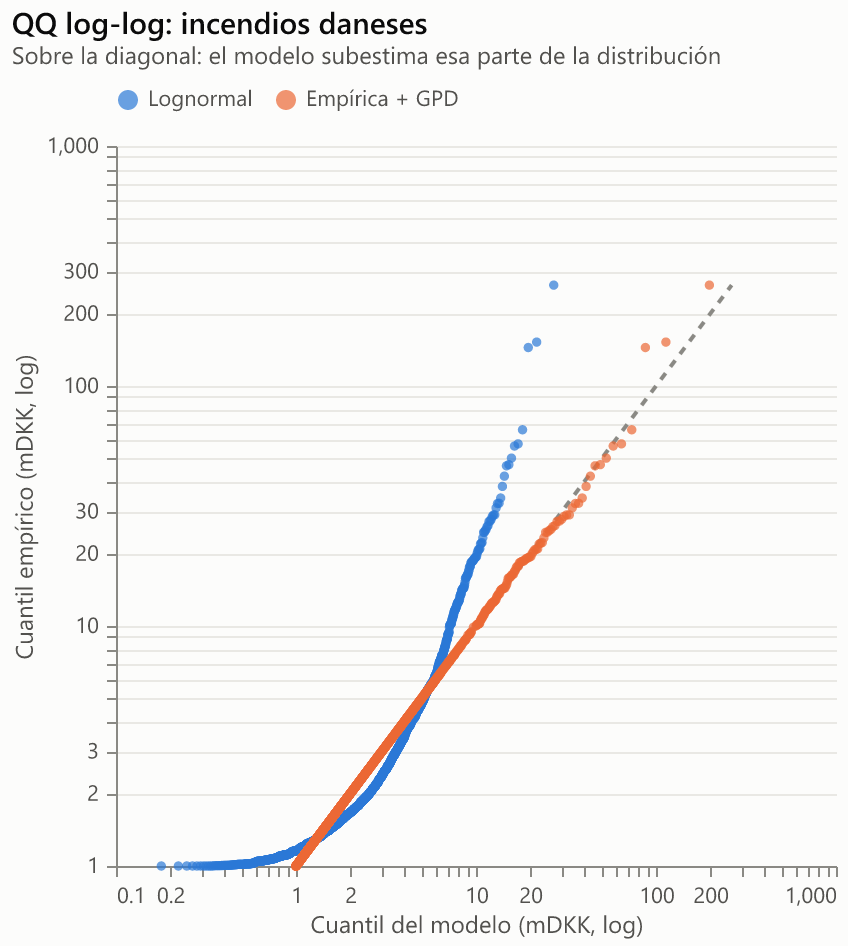
\includegraphics[width=.49\linewidth]{../figures/18_qq_dinamarca.png}\hfill
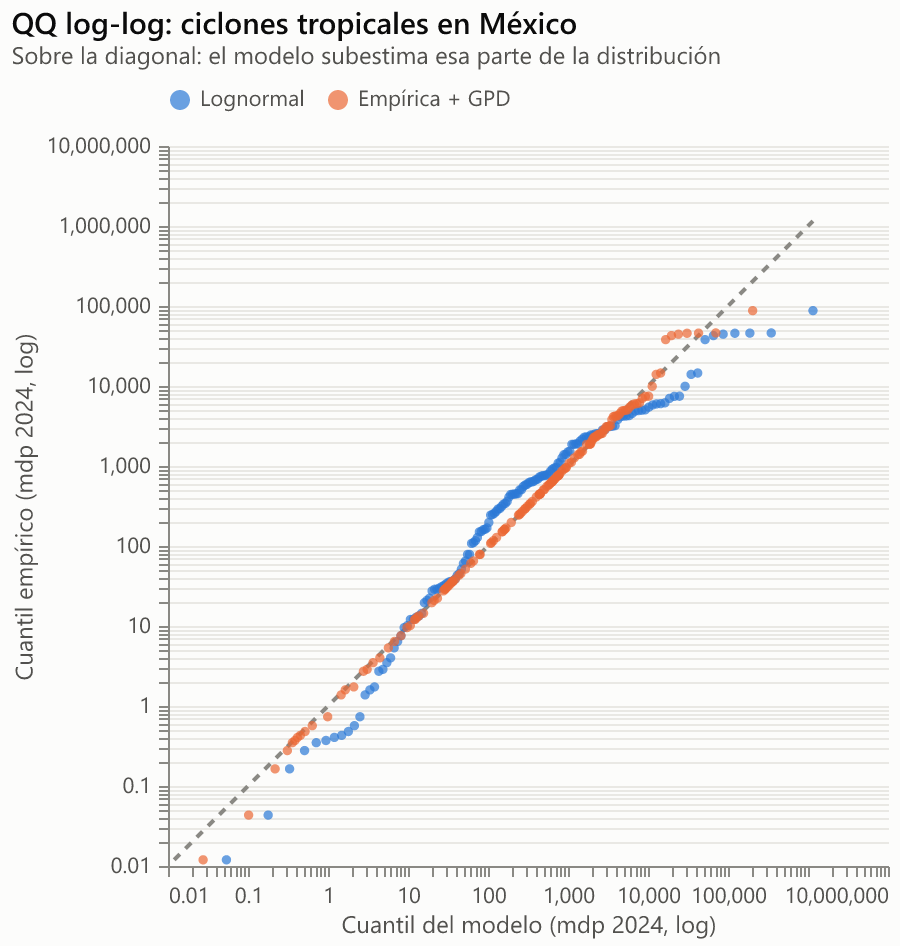
\includegraphics[width=.49\linewidth]{../figures/19_qq_mexico.png}
\caption{QQ en escala log-log (muestra completa). En la cola danesa los puntos de la lognormal quedan sobre la diagonal: subestima las pérdidas grandes. La GPD sigue la diagonal.}
\end{figure}

\subsection{Conclusión del problema}
Un buen ajuste \emph{central} (KS, QQ en el cuerpo, medianas) no garantiza nada en la \emph{cola}. La cola se valida con excedencias fuera de muestra, exceso medio y estabilidad de $\xi$ ante el umbral. Cuando la muestra es chica, como en México, la conclusión honesta es que \emph{los datos no discriminan}. En ese caso la decisión de reaseguro debe acompañarse de un análisis de sensibilidad a $\xi$ y a la pérdida máxima probable; el repositorio lo hace y obtiene prioridades óptimas entre 51\,300 y 143\,900 millones de pesos.

\appendix
\section{Programa de verificación}
Ejecución: \texttt{python notas/soluciones\_problemas.py}. El Problema 7 se reproduce con \texttt{python -m actuarial.problemas}.
\lstinputlisting[style=pyclean,caption={Verificación numérica de los Problemas 1 a 6.}]{soluciones_problemas.py}

\end{document}
